\chapter{Conception}
This chapter describes the concept and design of the application based on the previously analyzed requirements. This chapter outlines the application's structure, functionalities, technologies, and patterns used to fulfill the listed requirements.

\section{System Architecture}
In this section, an architecture diagram is displayed to have a better understanding of the system architecture as well as its components.
\begin{figure}[H]
    \centering
    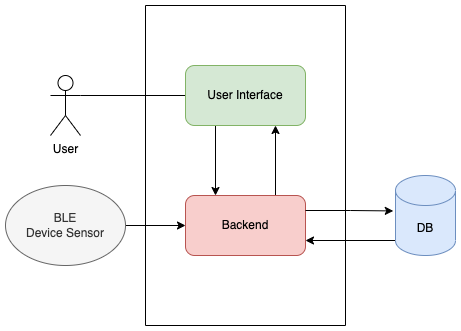
\includegraphics[width=1\textwidth]{diagrams/system-diagram.drawio.png}
    \caption{System architecture diagram}
    \label{fig:sys_diagram}
\end{figure}
\autoref{fig:sys_diagram} illustrates the components of the systems and the interaction between the components. Within the system, there are two components: the user interface and the backend which connects to a local database to store and manage data.
In addition, the device sensor is connected to the backend via bluetooth low energy and transmit the user's heart rate.
\section{Software Architecture}
This section serves as a guide to the high level structure of the application. It defines the key components as well as their relationship with each other.
Moreover, it describes the fundamental design patterns and architecture that define the application and its functionalities. 
The diagram presented below helps to gain better understanding of the application's architecture.
\begin{figure}[H]
    \centering
    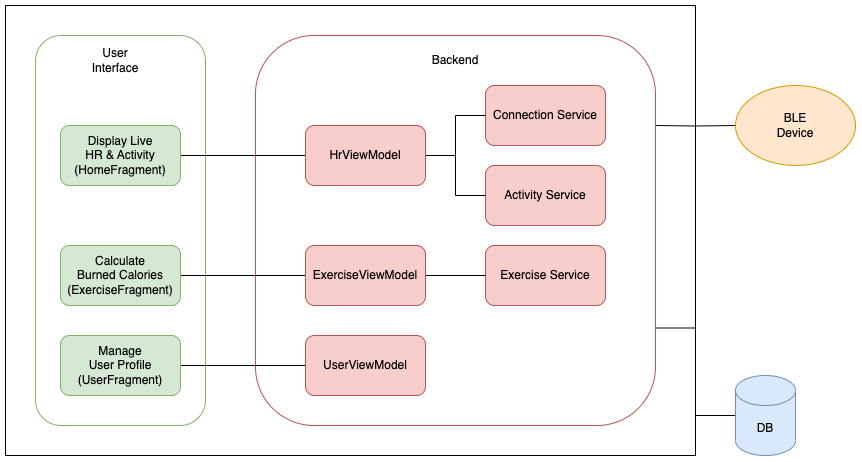
\includegraphics[width=1\textwidth]{diagrams/architecture-diagram.drawio.png}
    \caption{Software architecture diagram}
    \label{fig:soft_diagram}
\end{figure}
The project follows the Model-View-ViewModel (MVVM) architectural pattern. The user interface, which is responsible for displaying the features to the user, represents the \emph{view}. 
The \emph{model} is represented by the data and the business logic of the application, for instance, the entities and the functionalities such as live heart rate monitor, activity monitoring, exercise service, and user data management. 
The \emph{view model} facilitate the communications between the \emph{models} and the \emph{views} through which the \emph{views} can access and interact with the data and operations of the \emph{models}.

The user interface consists of three main components which extends \texttt{Fragment}\footnote{Based on The Official Android Documentation, a Fragment represents a reusable portion of your app's UI. A fragment defines and manages its own layout, has its own lifecycle, and can handle its own input events. \autocite{android-fragments}}. 
The \texttt{HomeFragment} displays real-time heart rate data and the activity monitor. It serves as the initial entry point for the users as they log in to the application. As it shows live heart rate data and activity, it holds a connection to the \texttt{HrViewModel}.
The \texttt{ExerciseFragment} presents the number of calories burned in an exercise based on the user's heart rate. It maintains a connection with the \texttt{ExerciseViewModel}. Lastly, the \texttt{UserFragment}, which is connected to the \texttt{UserViewModel}, displays the user's data and provide the necessary UI components to support data management.

The backend is in charge of the core functionalities of the application, which involve establishing a connection to the database.
As one of the core components, the \texttt{ConnectionService} maintains the connection between the BLE device and the application. It actively listens to the heart rate data being broadcasted by the BLE device. 
The \texttt{ActivityService} determines the current activity status based on the user's heart rate and age. 
On the other hand, the \texttt{ExerciseService} tracks the user's energy expenditure during training based on the user's heart rate and physical measurements such as weight, age, and gender. Both the \texttt{ExerciseService} and \texttt{ActivityService} subscribe to an event, where the heart rate data is published by the \texttt{ConnectionService}. This enables the services to receive the heart rate data seamlessly and process it accordingly.
Lastly, the \texttt{UserViewModel} is responsible for the management of the user's data and facilitates CRUD operations related to the user's data.



\section{Technologies}
Tech section
\subsection{User Interface}
talk about what tech is used for the ui
\subsection{Backend Infrastructure}
talk about what tech is used for the backend
\subsection{Database}
talk about what tech is used for the db
\subsection{BLE Sensor Device}
talk about what tech is used for the db


\section{Software Design}
the model-view-viewmodel follows the separation of concerns principles blablabla
The MVVM pattern promotes loose coupling and separation of concerns, making the application more maintainable and testable. The View and ViewModel are often connected using data binding techniques, allowing automatic synchronization of data between the two.
By following MVVM, developers can achieve a clear separation of responsibilities, allowing for easier development, testing, and maintenance of the application.
\subsection{Model}
\subsection{View}
\subsection{ViewModel}

% \section{Features}
